\chapter{Le \textit{pipeline} graphique}

\section{Introduction}
Avant de nous lancer dans l'étude de la programmation de \textit{fragment shaders}, il me semblait primordial de revenir rapidement sur le \textit{pipeline} de la carte graphique et ses différentes étapes afin d'avoir une meilleure compréhension de ce processus qui permet d'afficher une scène 3D sur un écran 2D.

\subsection*{Différences entre le GPU et le CPU}
Les différences fondamentales entre le CPU et le GPU résident principalement dans leurs architectures, leurs conceptions et leurs fonctions principales. Le CPU est conçu pour exécuter des tâches de manière séquentielle. Le \textit{strip} \ref{cpu00} illustre le processus de dessin d'une image \textit{pixel} par \textit{pixel} de manière séquentielle et lente. 

\begin{figure}[h]
  \begin{minipage}[b]{0.30\linewidth}
    \centering
    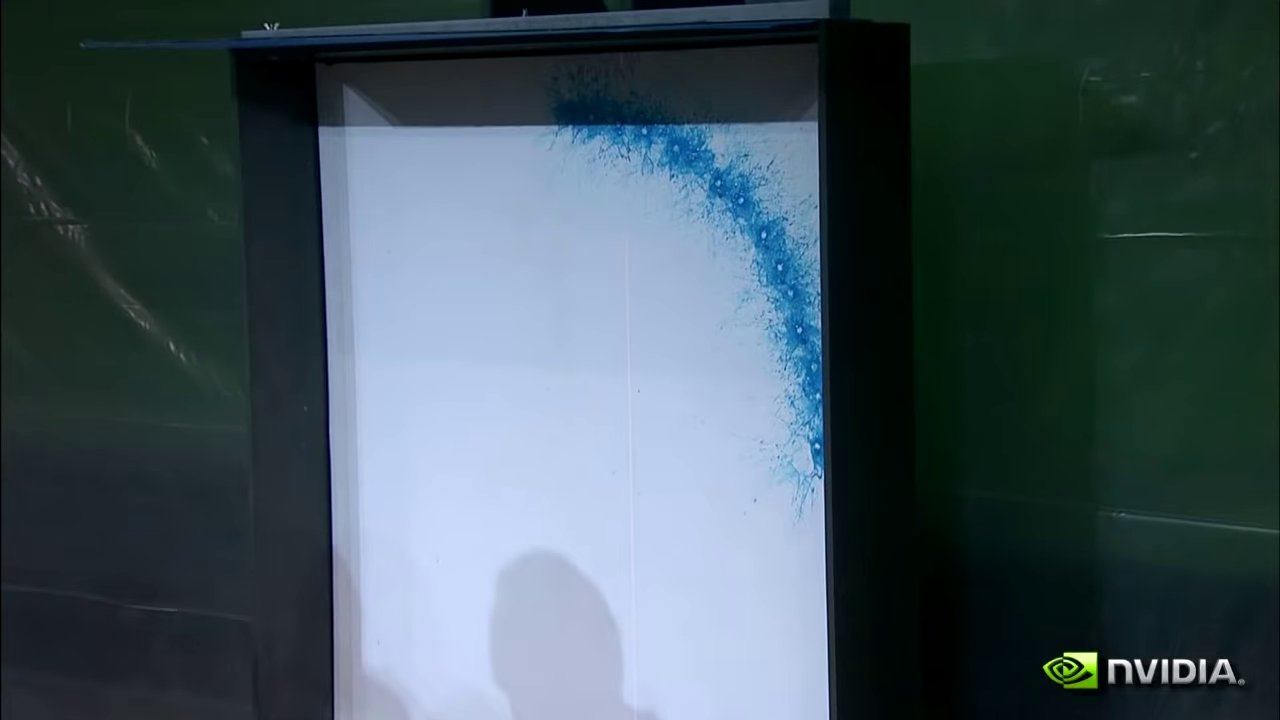
\includegraphics[width=\linewidth]{images/pipeline/gpu00.png}
  \end{minipage}
  \hfill
  \begin{minipage}[b]{0.30\linewidth}
    \centering
    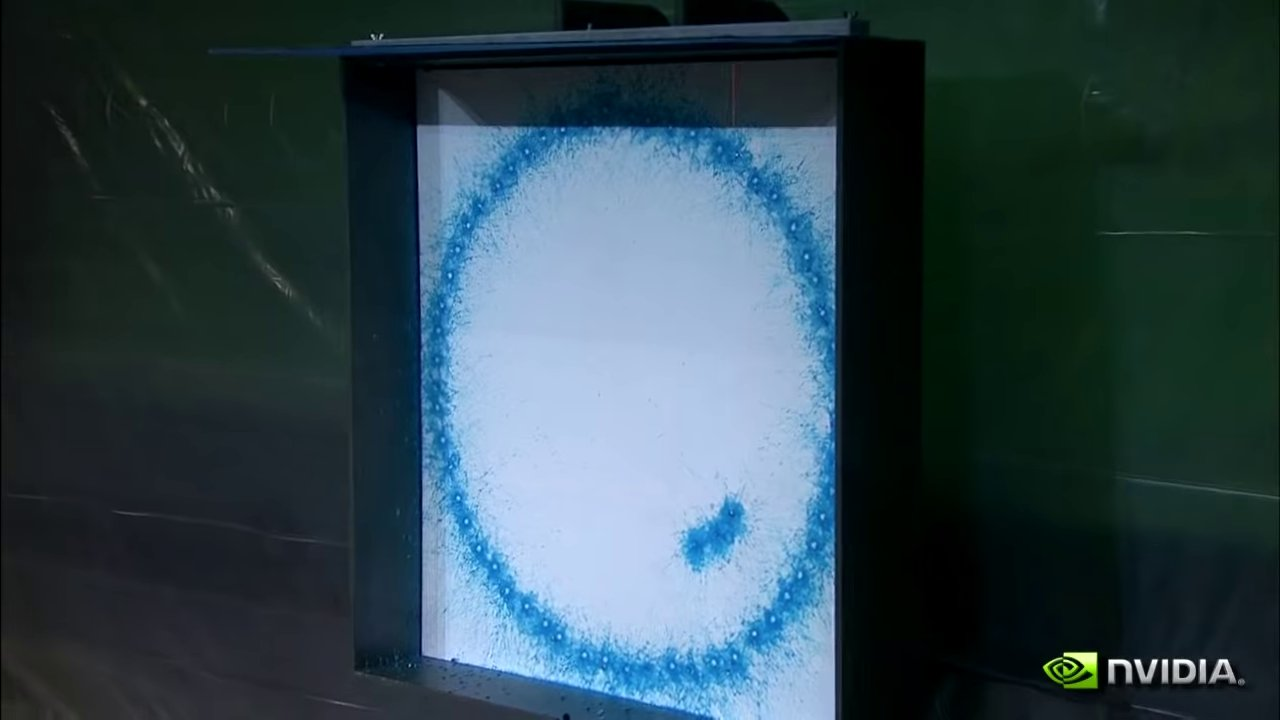
\includegraphics[width=\linewidth]{images/pipeline/gpu01.png}
  \end{minipage}
  \hfill
  \begin{minipage}[b]{0.30\linewidth}
    \centering
    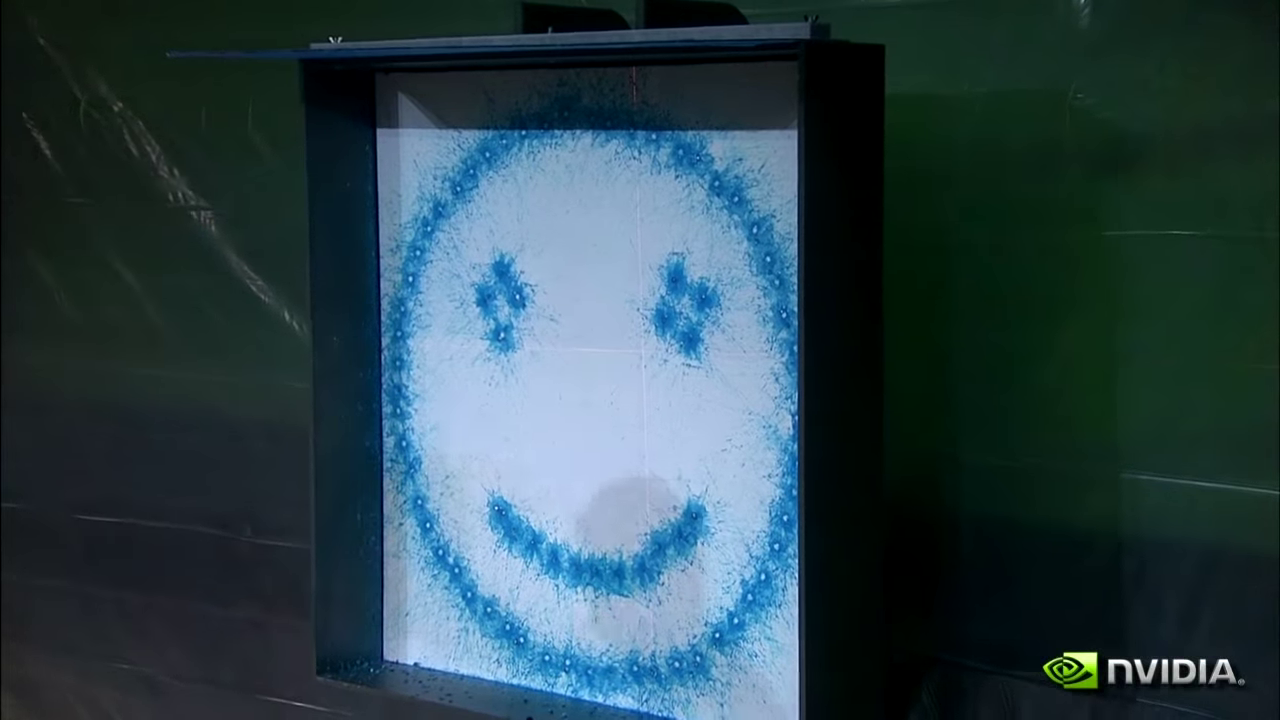
\includegraphics[width=\linewidth]{images/pipeline/gpu02.png}
  \end{minipage}
  \caption{Le CPU: intelligent mais lent}
  \label{cpu00}
\end{figure}

En revanche, le GPU est conçu avec un grand nombre de cœurs plus simples (parfois des milliers) qui peuvent travailler simultanément sur des tâches parallèles, offrant une capacité de traitement massivement parallèle pour les opérations graphiques. Le \textit{strip} \ref{gpuill} illustre bien cette caractéristique : le GPU est représenté par une grille de tuyaux qui envoient directement leurs informations sur chaque \textit{pixel} pour dessiner la Joconde en un instant. Ces \textit{strips} sont tirés d'une vidéo d'une \href{https://www.youtube.com/watch?app=desktop&v=WmW6SD-EHVY}{conférence humoristique de NVIDIA datant de 2008}.

\begin{figure}[h]
  \begin{minipage}[b]{0.30\linewidth}
    \centering
    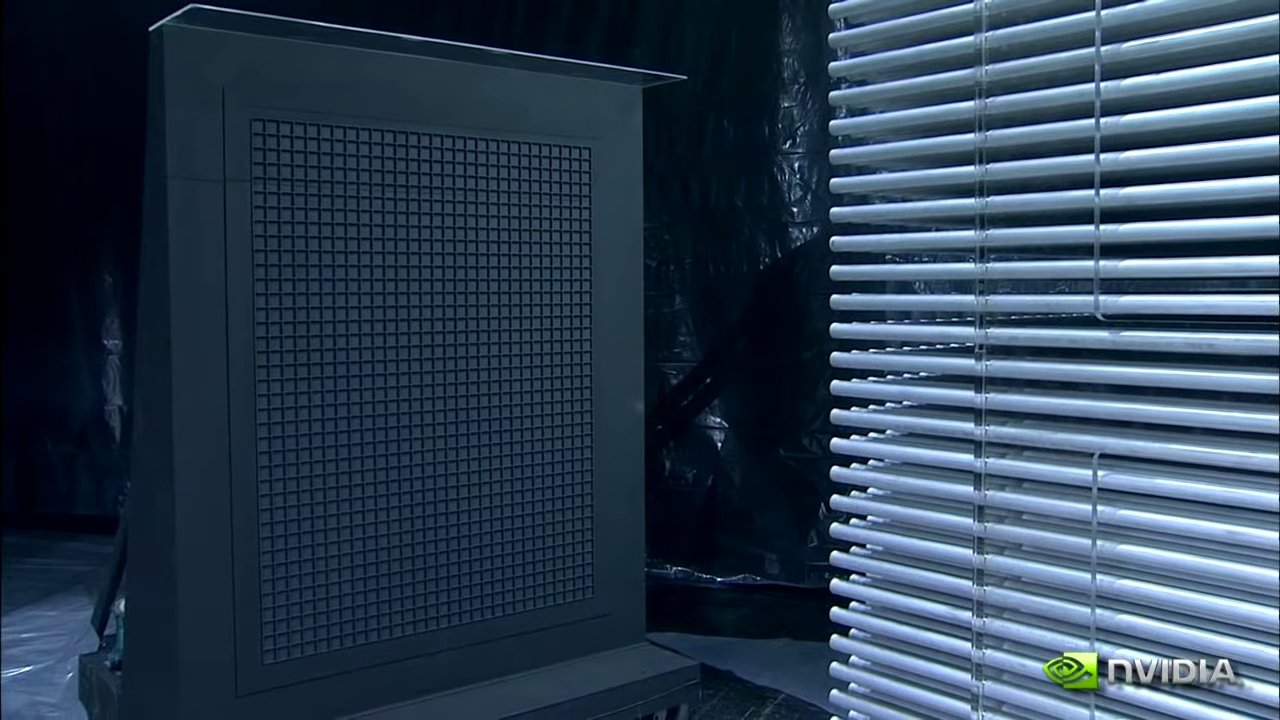
\includegraphics[width=\linewidth]{images/pipeline/gpu03.png}
  \end{minipage}
  \hfill
  \begin{minipage}[b]{0.30\linewidth}
    \centering
    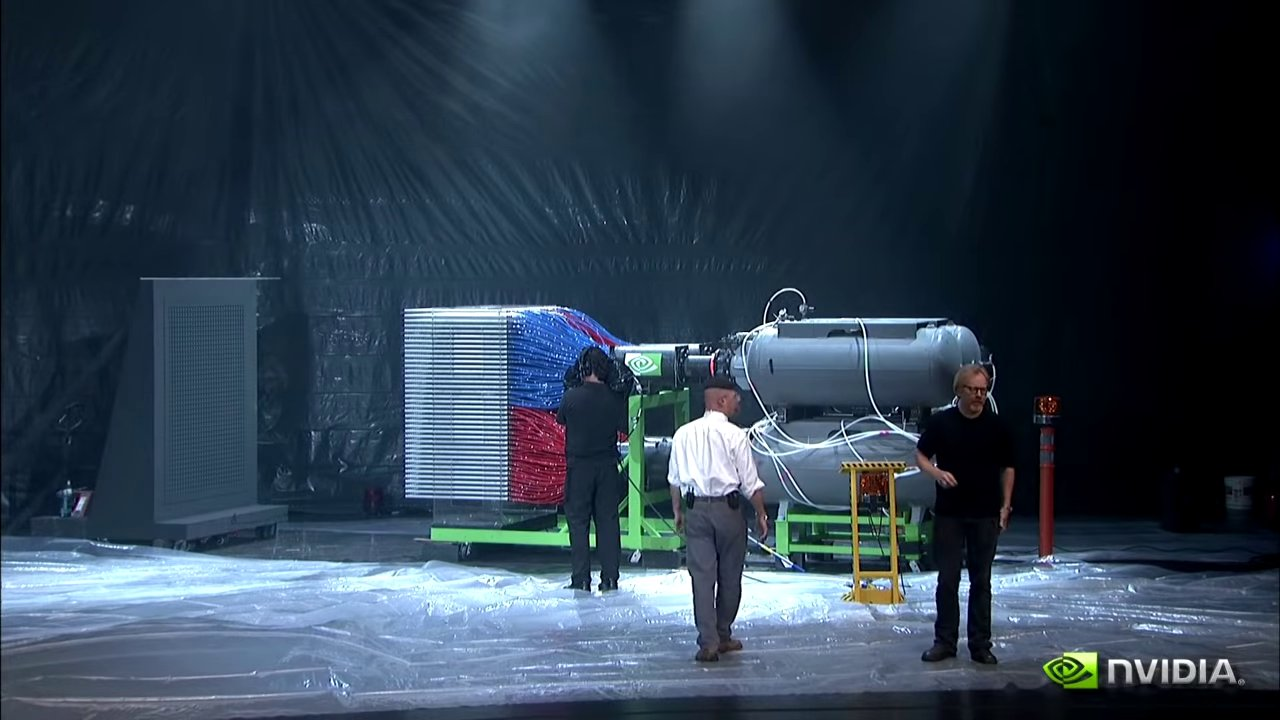
\includegraphics[width=\linewidth]{images/pipeline/gpu04.png}
  \end{minipage}
  \hfill
  \begin{minipage}[b]{0.30\linewidth}
    \centering
    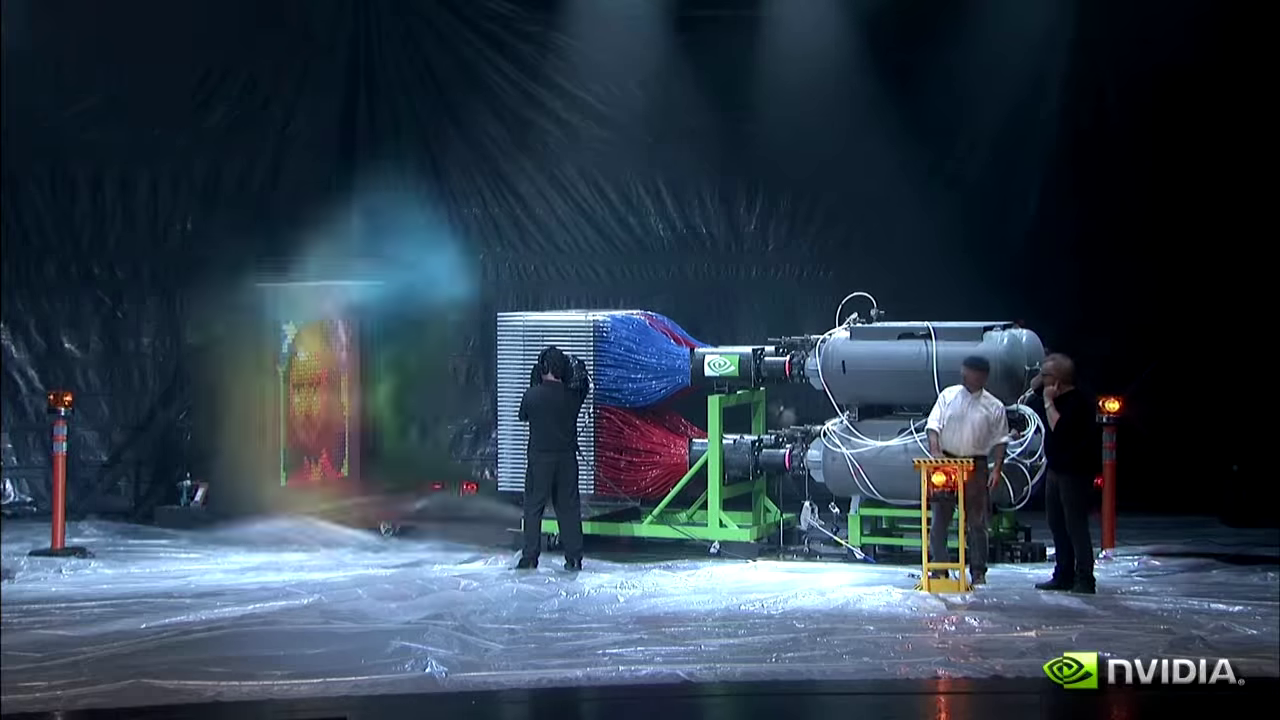
\includegraphics[width=\linewidth]{images/pipeline/gpu05.png}
  \end{minipage}
  \caption{Le GPU: rapide mais idiot}
  \label{gpuill}
\end{figure}


\subsection*{Comprendre le GPU}

D'ailleurs, lorsque l'on parle du \textit{pipeline} de la carte graphique c'est un abus de langage, on devrait plutôt parler de \textit{pipeline} du GPU (\textit{Graphical Processor Unit}). Schématiquement, une carte graphique se compose d'un processeur dédié, le GPU, et d'une mémoire vive spécifique (voir \ref{gpuproc}).

\begin{figure}[h]
  \begin{minipage}[b]{0.45\linewidth}
    \centering
    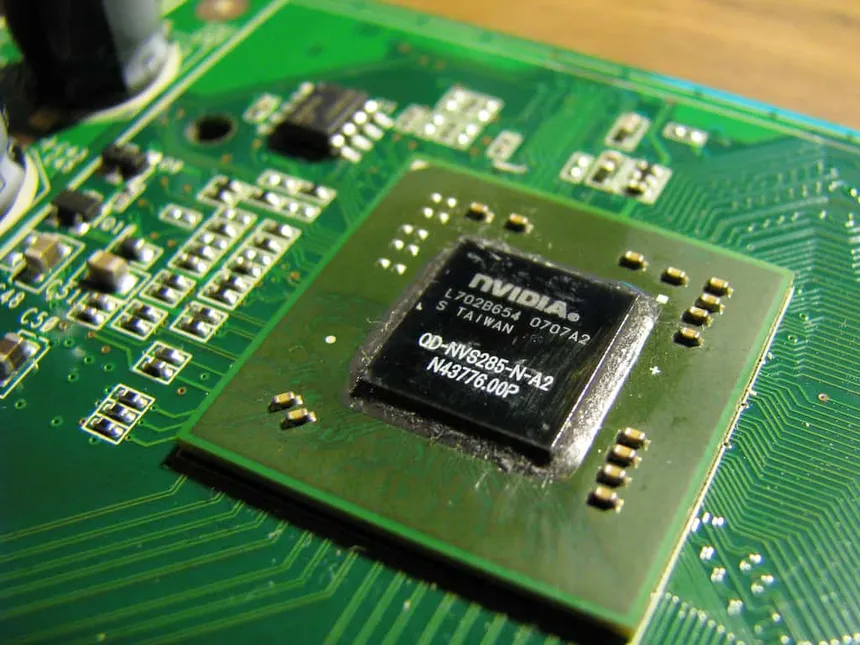
\includegraphics[width=0.75\linewidth]{images//shaders/gpu00.png}
    \label{gpu00}
  \end{minipage}
  \hspace{0.1\linewidth} % Espace horizontal pour la gouttière
  \begin{minipage}[b]{0.45\linewidth}
    \centering
    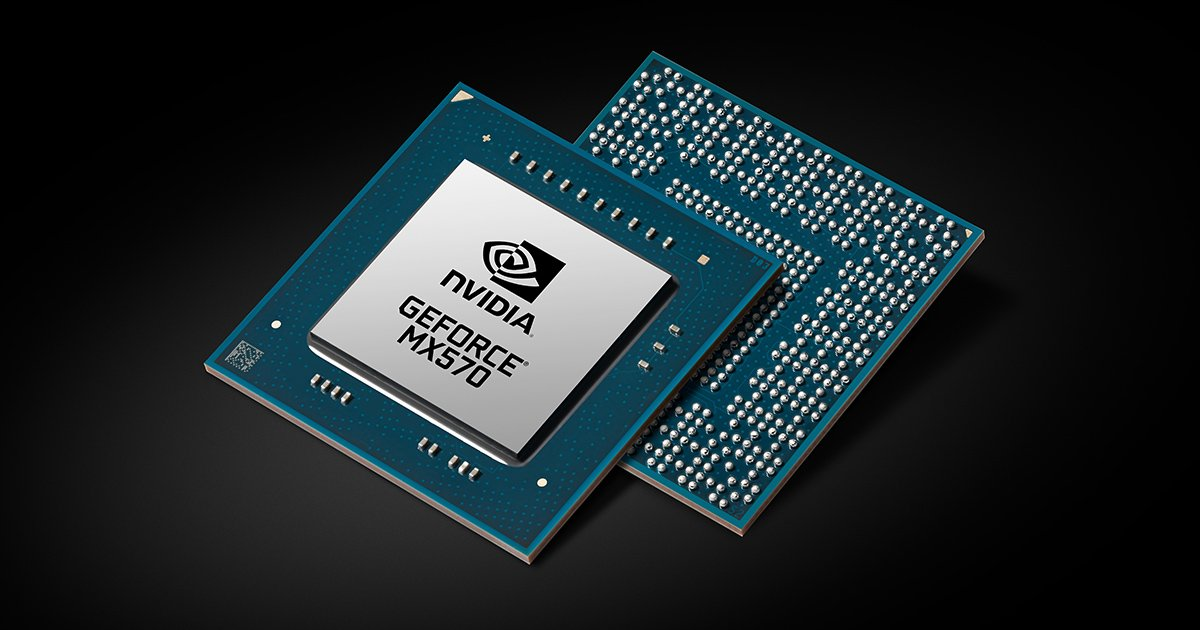
\includegraphics[width=0.75\linewidth]{images/pipeline/cg01.jpg}
    \label{gpu01}
  \end{minipage}
  \caption{Le GPU désigne le processeur dédié au traitement des données graphiques.}
  \label{gpuproc}
\end{figure}

Le rôle principal d'un GPU est de créer des images à partir de données qui décrivent la scène. En général, ces données en entrée sont une collection de triangles, car les triangles sont la forme géométrique atomique pour décrire un objet 3D: avec des triangles, nous pouvons représenter n'importe quel objet en trois dimensions. Avant de pouvoir être exploitées par le GPU, ces données représentant la scène (une collection de coordonnées de sommets\footnote{Un sommet (\textit{vertex} en anglais) est un point dans l'espace tridimensionnel. Les sommets sont des entités fondamentales utilisées pour définir la géométrie des objets dans une scène 3D. } représentant les triangles dans l'espace 3D) doivent être chargées dans la mémoire vive du GPU. Il faut donc que ces données soient décrites côté CPU avant de les envoyer au \textit{pipeline} de rendu (voir \ref{pipeline01} et \ref{gpu01comm}).

\begin{figure}[h]
  \begin{minipage}[b]{0.45\linewidth}
    \centering
    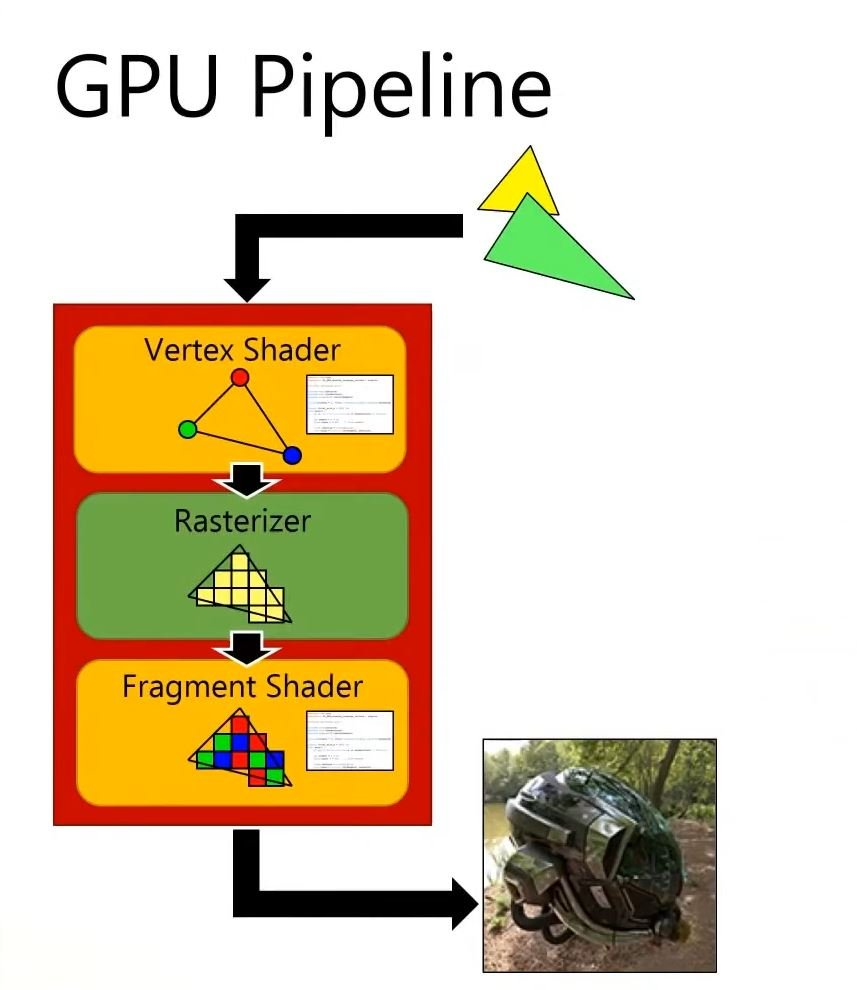
\includegraphics[width=0.75\linewidth]{images//shaders/pipeline01.jpg}
    \caption{Le pipeline graphique}
    \label{pipeline01}
  \end{minipage}
  \hspace{0.1\linewidth} % Espace horizontal pour la gouttière
  \begin{minipage}[b]{0.45\linewidth}
    \centering
    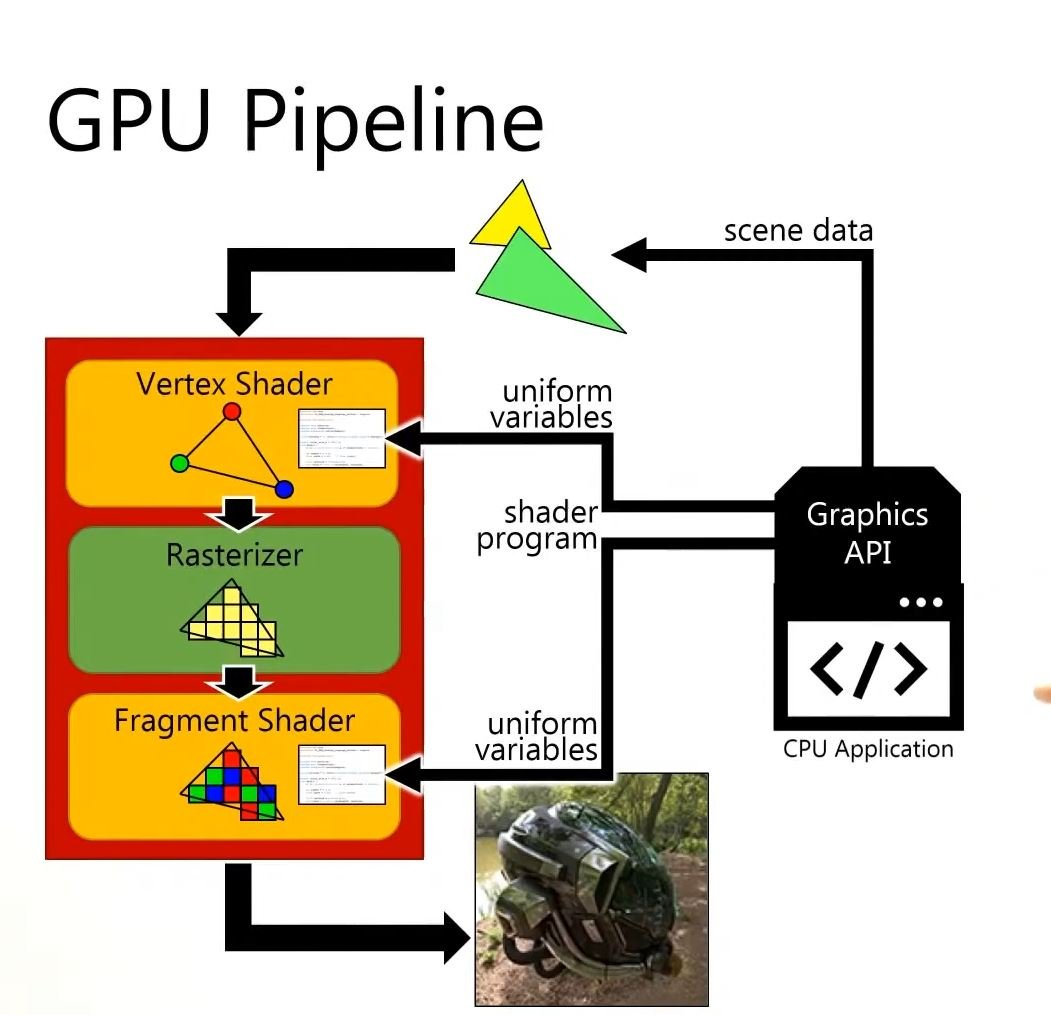
\includegraphics[width=0.75\linewidth]{images//shaders/pipeline02.jpg}
    \caption{Communication CPU-GPU}
    \label{gpu01comm}
  \end{minipage}
\end{figure}






\subsection*{Le parallélisme dans le GPU}   
Il faut voir la carte graphique comme une machine capable de parallélisme, c'est à dire qu'elle effectuera ses calculs sur chacun des sommets puis sur chacun des \textit{pixels} en parallèle. Le même \textit{vertex shader} s'exécutera une fois pour chaque \textit{vertex} et le même \textit{fragment shader} s'exécutera une fois pour chaque \textit{pixel} comme si la carte graphique possédait des tuyaux dédiés pour chaque \textit{pixel}. En d'autres termes, si l'écran a une résolution de $1920\times1080$, le \textit{fragment shader} devra être exécuté $2.073.600$ fois par image calculée. Les GPU peuvent gérer cela parce qu'ils colorient de nombreux \textit{pixels} en parallèle (c'est-à-dire en même temps) grâce à des \textit{threads}\footnote{Un \textit{thread} fait référence à une unité de traitement ou à une séquence d'instructions exécutées par le processeur graphique. Les GPU modernes sont équipés de multiples processeurs de flux, chacun capable de gérer plusieurs \textit{threads} simultanément.} dédiés aux calculs de chaque fragment. En particulier pour le \textit{fragment shader}, le programme ne peut agir que sur un seul \textit{pixel} à la fois et ne peut pas accéder aux valeurs des \textit{pixels} voisins. En cela on dit souvent que le \textit{shader} est aveugle. Il est aussi incapable de se souvenir du résultat du calcul de l'image précédente, en cela on parle d'amnésie du \textit{shader}.


\subsection*{Optimisation matérielle}
Un autre avantage du GPU est qu'il possède une accélération matérielle conçue pour optimiser certaines fonctions mathématiques utilisées couramment lors de l'écriture des \textit{shaders}, comme les opérations sur les matrices ou les calculs trigonométriques. 
% \todo{ajouter des petits exemples pour la forme, sin par exemple}





\section{Étapes du \textit{pipeline} graphique : du \textit{vertex} au \textit{fragment shader}}

Le \textit{pipeline} de traitement graphique assure la conversion des attributs des sommets en une image tridimensionnelle qui est ensuite affichée à l'écran. Les attributs habituels comprennent la coordonnée 3D de chaque sommet, sa coordonnée de texture et sa couleur. Cependant, il est possible d'ajouter n'importe quel attribut car la carte graphique interprétera ces données comme de la « data » pure. Les différentes étapes de ce \textit{pipeline}, dans leur séquence chronologique, comprennent le \textit{vertex shader}, le \textit{geometry shader}, la rastérisation (\textit{rasterization} en anglais) et le \textit{fragment shader}. Dans cette section, nous nous concentrerons sur une analyse détaillée du \textit{vertex shader}, du \textit{geometry shader} et de la rastérisation. Quant au \textit{fragment shader}, qui constitue la pierre angulaire du \textit{livecoding}, il sera décortiqué dans le prochain chapitre.


\subsection*{Le \textit{vertex shader}}

\subsubsection*{Le \textit{vertex shader} en code}
Voici un exemple très basique d'un \textit{vertex shader}. On peut remarquer que les données de la scène sont réceptionnées dans les variables \lstinline{pos} (3 coordonnées en $X$, en $Y$ et en $Z$) et \lstinline{col} (3 valeurs pour le rouge, le vert et le bleu et 1 valeur pour l'opacité). On a donc accès à la position et à la couleur de chaque \textit{vertex}.

\begin{minipage}{\linewidth}
\begin{lstlisting}[language=GLSL, caption=\textit{Vertex shader} en GLSL]
attribute vec3 pos;
attribute vec4 col;
void main()
{
  gl_Position = vec4(pos,1);
}
\end{lstlisting}
\end{minipage}

La variable \lstinline{gl_Position} est une variable de sortie, donc le programme se contente de récupérer la position de chaque \textit{vertex} et de l'envoyer à la prochaine étape du \textit{pipeline} (la rastérisation) sans leur appliquer de transformation. On remarque cependant l'ajout d'une quatrième composante avec la valeur $1$. Ce $1$ indique que nous utilisons des coordonnées homogènes\footnote{Les coordonnées homogènes sont un concept clé en géométrie et en informatique graphique, offrant une représentation unifiée des points et des vecteurs ainsi que des avantages significatifs pour les opérations géométriques et les transformations.}. En simplifiant on peut retenir que lorsque cette quatrième composante est à $1$ cela signifie que l'on désigne une position, et lorsqu'elle est à $0$ que l'on désigne une direction.

\subsection*{Comprendre les transformations matricielles}

Le rôle fondamental du \textit{vertex shader} est de transformer les coordonnées de chaque sommet dans différents espaces, comme nous l'explorerons plus en détail dans la section suivante. Heureusement, les matrices de transformation permettent d'appliquer facilement des opérations telles que la translation, la rotation et la mise à l'échelle sur des objets en 3D. Il est à noter qu'une quatrième composante, notée $w$, est utilisée pour décrire les coordonnées des sommets. Cette composante facilite la représentation des transformations projectives et simplifie les calculs mathématiques nécessaires au rendu 3D.

\subsubsection*{La matrice identité}
La matrice identité\footnote{La matrice identité est une matrice carrée dans laquelle tous les éléments de la diagonale principale sont égaux à $1$, tandis que tous les autres éléments sont égaux à $0$.} est couramment utilisée comme point de départ pour les transformations. En effet, elle permet de s'assurer du contenu de la mémoire avant d'effectuer les transformations matricielles. Elle agit comme un élément neutre pour la multiplication matricielle, comme le $0$ pour l'addition ou le $1$ pour la multiplication. Elle est souvent modifiée en ajoutant des opérations de translation, de rotation ou de mise à l'échelle pour produire des transformations plus complexes.
\[
\begin{bmatrix}
1 & 0 & 0 & 0\\
0 & 1 & 0 & 0\\
0 & 0 & 1 & 0\\
0 & 0 & 0 & 1
\end{bmatrix}
\cdot
\begin{bmatrix}
1\\
2\\
3\\
4
\end{bmatrix}
=
\begin{bmatrix}
1\\
2\\
3\\
4
\end{bmatrix}
\]

\subsubsection*{La matrice de mise à l'échelle}

Si nous remplaçons les $1$ de la matrice d'identité par des $3$, cela signifie que chaque élément du vecteur serait multiplié par $3$ lors de la multiplication matricielle. En conséquence, le vecteur serait uniformément augmenté de $3$ dans toutes les directions. En représentant les facteurs d'échelle par $(S1, S2, S3)$, nous pouvons définir une matrice d'échelle pour n'importe quel vecteur $(x, y, z)$ comme suit :
\[
\begin{bmatrix}
S1 & 0 & 0 & 0\\
0 & S2 & 0 & 0\\
0 & 0 & S3 & 0\\
0 & 0 & 0 & 1
\end{bmatrix}
\cdot
\begin{bmatrix}
x\\
y\\
z\\
1
\end{bmatrix}
=
\begin{bmatrix}
x \cdot S1\\
y \cdot S2\\
z \cdot S3\\
1
\end{bmatrix}
\]


\subsubsection*{La matrice de translation}

La translation déplace un objet d'une certaine distance le long des axes $X$, $Y$ et $Z$. Pour représenter une translation dans une matrice de transformation, on utilise une matrice identité de taille $4\times4$, mais avec des valeurs spécifiques dans la dernière colonne (les trois premières valeurs de la dernière colonne représentent les translations le long des axes $X$, $Y$ et $Z$ respectivement). Par exemple, pour une translation de $tx$, $ty$, $tz$, la matrice de transformation ressemblerait à cela :

\[
\begin{bmatrix}
1 & 0 & 0 & T_x\\
0 & 1 & 0 & T_y\\
0 & 0 & 1 & T_z\\
0 & 0 & 0 & 1
\end{bmatrix}
\cdot
\begin{bmatrix}
x\\
y\\
z\\
1
\end{bmatrix}
=
\begin{bmatrix}
x + T_x\\
y + T_y\\
z + T_z\\
1
\end{bmatrix}
\]

\subsubsection*{La matrice de rotation autour de l'axe X}
La rotation fait tourner un objet autour des axes $X$, $Y$ et $Z$. Les rotations peuvent être définies en radians ou en degrés. Pour chaque axe de rotation, il existe une matrice de rotation correspondante. Par exemple, pour une rotation autour de l'axe $X$ par un angle $\theta$, la matrice de rotation serait :
\[
\begin{bmatrix}
1 & 0 & 0 & 0\\
0 & \cos{\theta} & -\sin{\theta} & 0\\
0 & \sin{\theta} & \cos{\theta} & 0\\
0 & 0 & 0 & 1
\end{bmatrix}
\cdot
\begin{bmatrix}
x\\
y\\
z\\
1
\end{bmatrix}
=
\begin{bmatrix}
x\\
\cos{\theta} \cdot y - \sin{\theta} \cdot z\\
\sin{\theta} \cdot y + \sin{\theta} \cdot z\\\\
1
\end{bmatrix}
\]

\subsubsection*{La matrice de rotation autour de l'axe Y}
Pour la matrice de rotation autour de l'axe $Y$, on observe que cette matrice est semblable à celle de la rotation autour de l'axe $X$, à la différence près que des zéros ont été insérés dans la deuxième ligne et la deuxième colonne, à l'exception de la diagonale où un $1$ est conservé pour maintenir la position inchangée.

\[
\begin{bmatrix}
\cos{\theta} & 0 & \sin{\theta} & 0\\
0 & 1 & 0 & 0\\
-\sin{\theta} & 0 & \cos{\theta} & 0\\
0 & 0 & 0 & 1
\end{bmatrix}
\cdot
\begin{bmatrix}
x\\
y\\
z\\
1
\end{bmatrix}
=
\begin{bmatrix}

\cos{\theta} \cdot x + \sin{\theta} \cdot z\\
y\\
-\sin{\theta} \cdot x + \cos{\theta} \cdot z\\
1
\end{bmatrix}
\]

\subsubsection*{La matrice de rotation autour de l'axe Z}
Le même phénomène se produit pour la rotation autour de l'axe $Z$ mais avec la troisième ligne et la troisième colonne.

\[
\begin{bmatrix}
\cos{\theta} & -\sin{\theta} & 0 & 0\\
\sin{\theta} &  \cos{\theta} & 0 & 0\\
0 & 0 & 1 & 0\\
0 & 0 & 0 & 1
\end{bmatrix}
\cdot
\begin{bmatrix}
x\\
y\\
z\\
1
\end{bmatrix}
=
\begin{bmatrix}
\cos{\theta} \cdot x - \sin{\theta} \cdot y\\
\sin{\theta} \cdot x + \cos{\theta} \cdot y\\
z\\
1
\end{bmatrix}
\]

\subsection*{Comprendre les systèmes de coordonnées en 3D}

Il était utile d'aborder le fonctionnement des matrices de transformation, car le \textit{vertex shader} a pour objectif de convertir efficacement une représentation spatiale en une autre. Le rôle principal du \textit{vertex shader} est de transformer les coordonnées 3D de notre objet en coordonnées 3D normalisées\footnote{Les coordonnées 3D normalisées (NDC), abréviation de \textit{Normalized Device Coordinates} en anglais, sont un système de coordonnées tridimensionnelles utilisé dans les graphiques 3D. Dans ce système, les coordonnées sont normalisées par rapport à la taille de l'espace de visualisation, de sorte que les coordonnées $X$, $Y$ et $Z$ varient toutes entre $-1$ et $1$.} qui s'afficheront à l'écran. Ces coordonnées doivent se situer dans l'intervalle $[-1, 1]$, car les sommets avec des coordonnées en dehors de cette plage ne seront pas visibles à l'écran. Le problème dans le code précédent est que nous nous contentons de passer les coordonnées 3D des sommets sans appliquer de transformation. La transformation des coordonnées en NDC se fait étape par étape, en passant par cinq systèmes de coordonnées différents :

\begin{samepage}
\begin{enumerate}
    \item Coordonnées du modèle (\textit{Model Space})
    \item Coordonnées du monde (\textit{World Space})
    \item Coordonnées de la vue (\textit{View Space} ou \textit{Eye Space})
    \item Coordonnées de projection (\textit{Clip Space})
    \item Coordonnées normalisées de l'écran (NDC)
\end{enumerate}
\end{samepage}

Le \textit{vertex shader} est responsable de la transformation des coordonnées du modèle en coordonnées normalisées de l'écran, en appliquant une série de transformations matricielles appropriées à chaque sommet de l'objet (voir \ref{syscoord00}). Effectivement, chaque étape de transformation des coordonnées vers les coordonnées normalisées de l'écran s'appuie sur des matrices de transformation, parmi lesquelles figurent les matrices de modèle, de vue et de projection. 

\begin{figure}[h]
    \centering
    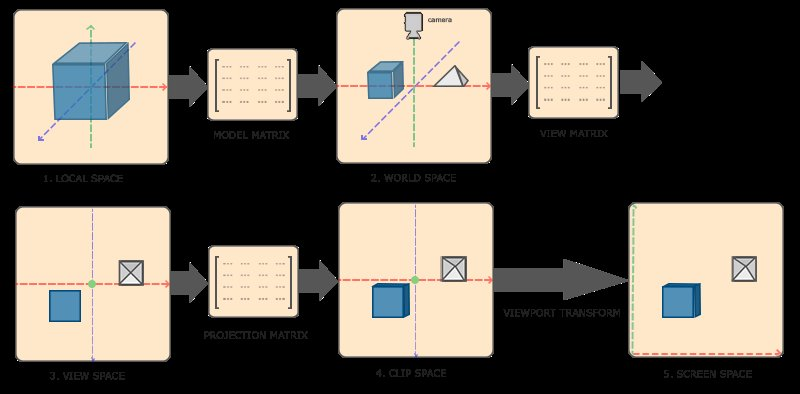
\includegraphics[width=0.75\linewidth]{images//shaders/syscoord00.png}
    \caption{Transformation des coordonnées dans le \textit{vertex shader}}
    \label{syscoord00}
\end{figure}

Initialement, nous disposons des coordonnées locales de notre objet par rapport à son origine locale. L'espace local représente les coordonnées locales de l'objet, c'est-à-dire l'endroit où il est créé ou modélisé. Par exemple, si nous créons un cube dans un logiciel de modélisation comme Blender, ce cube sera généralement centré autour de l'origine de l'espace local. 

Dans l'espace local, les coordonnées de chaque sommet sont définies par rapport au centre de l'objet. Cependant, pour rendre cet objet dans une scène 3D, nous devons le placer et l'orienter par rapport à la scène globale. C'est là que la matrice de modèle entre en jeu : elle permet de transformer les coordonnées locales de l'objet en coordonnées du monde, en appliquant des transformations telles que la translation, la rotation et la mise à l'échelle. Une fois que les coordonnées sont dans l'espace du monde, elles sont transformées dans l'espace de vue (ou espace œil) à l'aide de la matrice de vue. 

Dans cet espace, la caméra est positionnée à l'origine et les objets sont positionnés et orientés par rapport à la caméra. Cette transformation permet de simuler le déplacement et l'orientation de la caméra dans la scène. 

Ensuite, les coordonnées de vue sont transformées dans l'espace de projection à l'aide de la matrice de projection. Dans cet espace, les coordonnées sont projetées dans un espace 3D canonique, où les coordonnées $X$, $Y$ et $Z$ sont normalisées et se trouvent dans la plage $[-1, 1]$. Cette étape permet de déterminer quels objets sont visibles à l'écran et on peut utiliser soit la projection en perspective, soit la projection orthographique. Enfin, les coordonnées de projection sont transformées en coordonnées normalisées de l'écran (NDC) en divisant les coordonnées par leur composante $w$ (homogène). Cela place les coordonnées dans une plage standardisée de $[-1, 1]$, ce qui permet de déterminer quels sommets et quelles parties de la scène seront rendus à l'écran. Le volume qui détermine si un sommet sera affiché ou non s'appelle le \textit{frustum}\footnote{En informatique graphique, le \textit{frustum} est une approximation de la zone de l'espace tridimensionnel qui est visible à travers une caméra ou une fenêtre de visualisation. Il est utilisé pour décider quels éléments doivent être rendus dans une scène 3D.}.




Nous venons de mentionner qu'il existe deux types principaux de matrices de projection : la matrice de projection orthographique et la matrice de projection en perspective. Contrairement à la projection perspective , où les objets plus éloignés sont réduits en taille, la projection orthographique conserve la taille relative des objets, indépendamment de leur distance par rapport à la caméra. Cela signifie que les objets éloignés apparaissent de la même taille que les objets proches. La projection orthographique, quant à elle, est souvent utilisée dans les rendus 2D et dans certaines applications architecturales ou d'ingénierie où l'on souhaite éviter les déformations des objets dues à la perspective. Elle offre une représentation plus fidèle des dimensions et des proportions des objets, ce qui peut être préférable dans certains cas d'utilisation. Une application comme Blender, qui est utilisée pour la modélisation 3D, utilise parfois la projection orthographique pour la modélisation car elle représente plus précisément les dimensions de chaque objet (voir \ref{syscoord5}).

\begin{figure}[h]
    \centering
    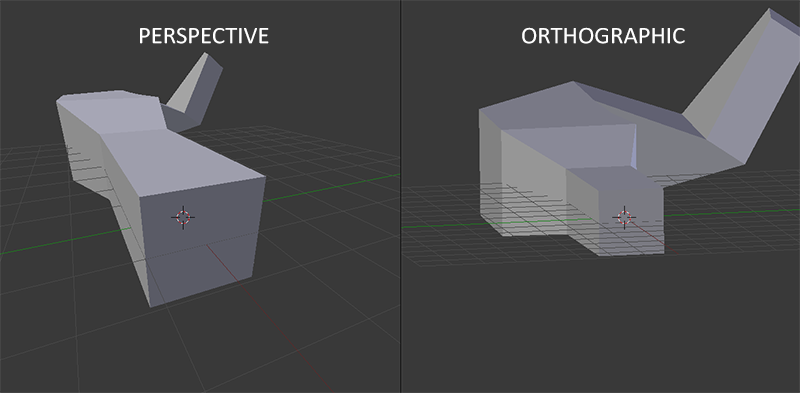
\includegraphics[width=0.75\linewidth]{images//shaders/syscoord5.png}
    \caption{Les deux types de projection dans Blender}
    \label{syscoord5}
\end{figure}


Dans le processeur central (CPU), après avoir défini une matrice de transformation pour chacune des étapes susmentionnées (modèle, vue et projection), on transforme les coordonnées de chaque sommet en coordonnées de l'espace NDC comme suit:

\begin{minipage}{\linewidth}
\begin{lstlisting}[language=GLSL, caption=\textit{Vertex shader} en GLSL]
attribute vec3 pos;
attribute vec4 col;
void main()
{
  gl_Position = m_proj * m_view * m_model * pos;
}
\end{lstlisting}
\end{minipage}

\subsection*{Le \textit{geometry shader}}

Le \textit{geometry shader} (ou nuanceur de géométrie en français) est aussi une étape programmable mais optionnelle qui se situe entre le \textit{vertex shader} et le \textit{fragment shader}. Le \textit{geometry shader} prend en entrée un ensemble de sommets qui forment une primitive unique, par exemple un point ou un triangle. Le \textit{geometry shader} peut ensuite transformer ces sommets comme il l'entend avant de les envoyer à l'étape suivante du \textit{pipeline}. Ce qui rend le \textit{geometry shader} intéressant, c'est qu'il est capable de convertir la primitive d'origine (ensemble de sommets) en des primitives complètement différentes, en générant éventuellement plus de sommets qu'il n'y en avait au départ.

Il peut par exemple subdiviser un \textit{quad}\footnote{En modélisation 3D, un \textit{quad}, abréviation de « quadrilatère », fait référence à un polygone composé de quatre sommets reliés par des arêtes.} pour créer de nouveaux triangles et ainsi donner plus de détails à la modélisation. On peut aussi s'en servir pour créer des formes complexes à partir de formes très simples. Par exemple, on peut créer un cheveu à partir d'un segment constitué de seulement deux sommets. En général, on l'utilise pour des effets visuels en temps réel tels que la déformation de la géométrie, la génération de particules, l'effet de feuillage pour les arbres, les vagues dans l'eau, etc.

\begin{figure}[h]
  \begin{minipage}[b]{0.45\linewidth}
    \centering
    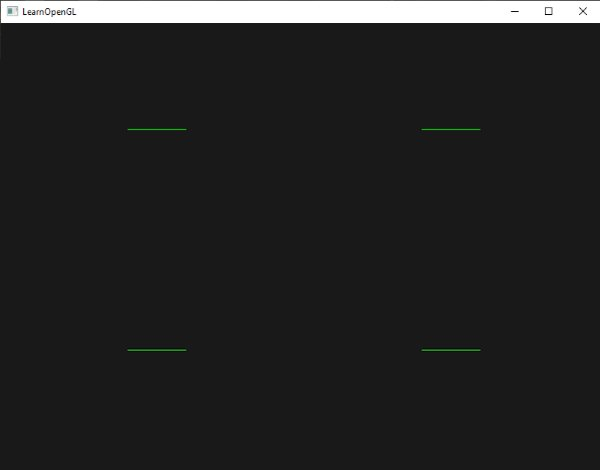
\includegraphics[width=\linewidth]{images/shaders/geometry_shader_00.png}
    \caption{\textit{Geometry shader} - Création d'un segment}
    \label{geo00}
  \end{minipage}
  \hspace{0.1\linewidth} % Espace horizontal pour la gouttière
  \begin{minipage}[b]{0.45\linewidth}
    \centering
    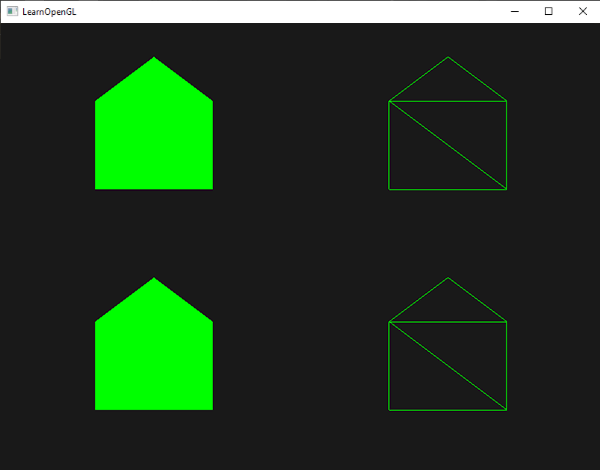
\includegraphics[width=\linewidth]{geometry_shader_01.png}
    \caption{\textit{Geometry shader} - Création d'une maison}
    \label{geo01}
  \end{minipage}
\end{figure}


Comme illustré plus haut (voir \ref{geo00}), le \textit{geometry shader} prend une primitive de point comme entrée et crée une primitive de ligne horizontale avec le point d'entrée en son centre. Au départ nous avions seulement quatre points provenant du CPU, et le \textit{geometry shader} à créé de nouveaux points pour chacun et empaqueté le tout dans une nouvelle primitive \lstinline{LINE} avant de l'envoyer aux étapes suivantes du \textit{pipeline}. Bien qu'il s'agisse d'un exemple relativement simple, il montre comment nous pouvons utiliser les \textit{geometry shaders} pour générer dynamiquement de nouvelles formes à la volée. Rien ne nous empêche de complexifier la tâche du \textit{geometry shader}. Dans le code suivant, à partir d'un seul point nous dessinons une maison en créant cinq nouveaux sommets (voir \ref{geo01}):

\begin{minipage}{\linewidth}
\begin{lstlisting}[language=GLSL, caption=\textit{Geometry shader} en GLSL - Maison à partir d'un seul \textit{vertex}]
#version 330 core
layout (points) in;
layout (triangle_strip, max_vertices = 5) out;

void build_house(vec4 position)
{    
    gl_Position = position + vec4(-0.2, -0.2, 0.0, 0.0);    // 1:bottom-left
    EmitVertex();   
    gl_Position = position + vec4( 0.2, -0.2, 0.0, 0.0);    // 2:bottom-right
    EmitVertex();
    gl_Position = position + vec4(-0.2,  0.2, 0.0, 0.0);    // 3:top-left
    EmitVertex();
    gl_Position = position + vec4( 0.2,  0.2, 0.0, 0.0);    // 4:top-right
    EmitVertex();
    gl_Position = position + vec4( 0.0,  0.4, 0.0, 0.0);    // 5:top
    EmitVertex();
    EndPrimitive();
}

void main() {    
    build_house(gl_in[0].gl_Position);
}  
\end{lstlisting}
\end{minipage}



\subsection*{Le \textit{rasterizer}}
La rastérisation est une étape cruciale du \textit{pipeline} graphique dans le processus de rendu en 3D. C'est l'étape qui consiste à convertir toutes les données 3D en une image matricielle en deux dimensions afin de pouvoir les afficher à l'écran (voir \ref{rasterizer}). Pour résumer, la rastérisation prend entrée la liste des triangles de l'étape précédente (espace 3D) et les convertit en \textit{pixels} (ou plus exactement des fragments) correspondant à chacun des triangles (espace 2D). C'est aussi lors de cette étape qu'une interpolation des attributs des sommets (tels que les couleurs, les coordonnées de texture, etc.) est effectuée sur les \textit{pixels} résultants. Le développeur n'a aucun contrôle sur cette étape, c'est un élément \textit{hardware} de la carte graphique qui est dédié à ces calculs : le \textit{rasterizer}.


\begin{figure}[h]
  \begin{minipage}[b]{0.45\linewidth}
    \centering
    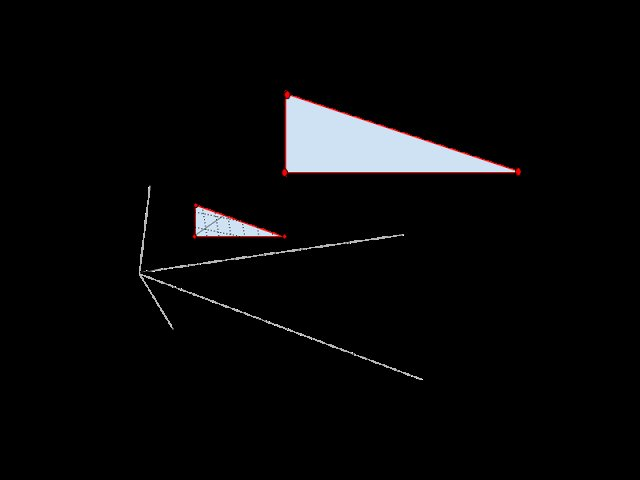
\includegraphics[width=\linewidth]{images/shaders/raster00.png}
  \end{minipage}
  \hspace{0.1\linewidth} % Espace horizontal pour la gouttière
  \begin{minipage}[b]{0.45\linewidth}
    \centering
    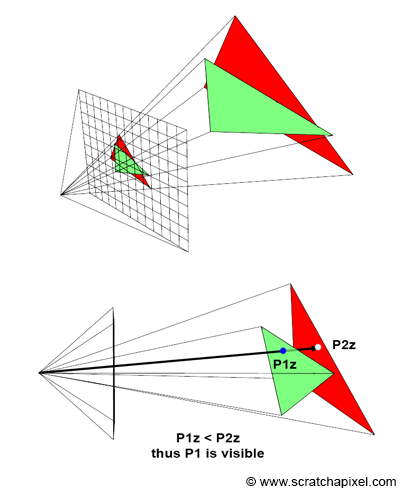
\includegraphics[width=\linewidth]{images/shaders/rasterizer.png}
  \end{minipage}
  \caption{Rastérisation}
  \label{rasterizer}
\end{figure}

\subsubsection*{Interpolation des attributs lors de la rastérisation}

Même si la couleur a été définie pour chaque \textit{vertex}, lorsque l'on se trouve à l'intérieur du \textit{fragment shader} c'est une valeur interpolée que l'on reçoit. Depuis le CPU, on associe des attributs aux \textit{vertices}: pour l'ordinateur il s'agit simplement de data. À un seul \textit{vertex}, en général on lui associe une position, une couleur, et une coordonnée d'uv. Ces données sont ensuite envoyées au GPU qui se chargera d'interpoler les valeurs via le \textit{rasterizer}. Ainsi, si l'on décrit un triangle dans le CPU, avec du rouge du vert du bleu associé à chacun de ses \textit{vertex}, le GPU affichera un triangle aux couleurs interpolées. Tous les \textit{pixels} situés à l'intérieur de ce triangle posséderont une couleur qui sera la combinaison des trois couleurs de chaque sommet, la quantité variant selon la distance par rapport à ces sommets.

\begin{figure}[h]
  \begin{minipage}[b]{0.40\linewidth}
    \centering
    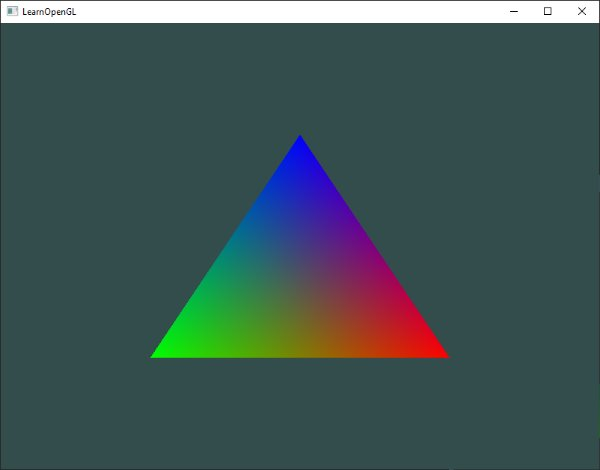
\includegraphics[width=\linewidth]{images/shaders/interpolation00.png}
    \label{interpolation00}
  \end{minipage}
  \hspace{0.1\linewidth} % Espace horizontal pour la gouttière
  \begin{minipage}[b]{0.40\linewidth}
    \centering
    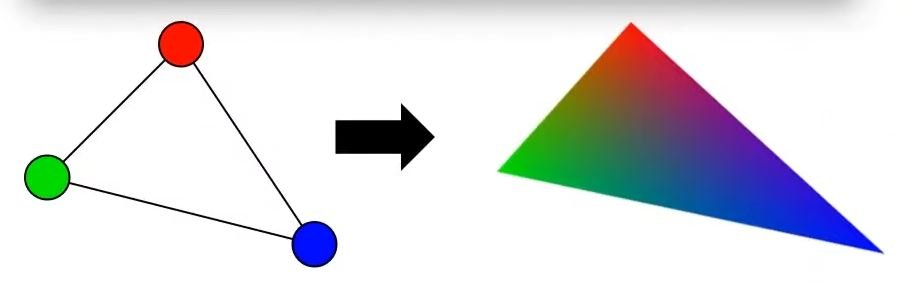
\includegraphics[width=\linewidth]{images/shaders/interpolation01.JPG}
    \label{interpolation01}
  \end{minipage}
  \caption{Interpolation des couleurs}
\end{figure}


\section{Conclusion}

Dans ce chapitre, nous avons plongé dans le cœur même du processus de rendu graphique en explorant le \textit{pipeline} graphique. Nous avons commencé par une revue du \textit{pipeline} de la carte graphique, de la compréhension du GPU à son architecture optimisée. Ensuite, nous avons parcouru les étapes essentielles du \textit{pipeline} graphique, en nous concentrant particulièrement sur le \textit{vertex shader} et le \textit{geometry shader}. Le \textit{vertex shader} joue un rôle indispensable en transformant les coordonnées des sommets dans différents espaces, tandis que le \textit{geometry shader} offre une flexibilité supplémentaire en permettant la création dynamique de géométrie. Enfin, nous avons examiné l'étape de rastérisation, où les primitives 3D sont converties en fragments 2D prêts à être affichés à l'écran. En combinant ces différentes étapes, le \textit{pipeline} graphique accomplit la tâche complexe de convertir des données 3D en une image 2D qui s'affiche sur nos écrans.

Nous allons consacrer le prochain chapitre à une étape fondamentale du \textit{pipeline} que nous n'avons volontairement pas traitée dans cette section : le \textit{fragment shader}. Cette étape revêt une importance capitale dans la pratique du \textit{livecoding}. Nous examinerons en détail les techniques essentielles à maîtriser pour une performance scénique réussie.



% \todo{à déplacer}
% \section{Fragment shader}

% Ensuite pour chacun des \textit{pixels}, on effectue une série d'opérations dans le fragment shader qui permet de calculer la couleur finale du \textit{pixel} qui apparaîtra au rendu.

% Le fragment shader est aussi utilisé pour des opérations plus complexes comme le calcul de l'éclairage et des ombres, le rendu d'une matière translucide ou encore pour le calcul de passes de post-processing comme le flou ou les aberrations chromatiques.

% \subsection{Fragment shader en code}
% On récupère la couleur de chaque vertex grâce à la variable \lstinlineplain{vcolor} définie précédemment dans le vertex shader et c'est elle qu'on utilisera pour colorier nos \textit{pixels}. 

% \lstinlineplain{gl_FragColor} est une variable de sortie définie dans OpenGL qui décrit la couleur finale de chaque \textit{pixel}. 

% \begin{lstlisting}[language=GLSL, caption=Fragment shader en GLSL - coloration]
% precision mediump float;
% varying vec4 vcolor;

% \todo{a déplacer}
% \subsection{API OpenGL}
% Pour faire communiquer le CPU avec le GPU on utilise une API graphique, une des plus connues étant OpenGL (d'autres solutions existent comme Vulkan , WebGL ou DirectX). Depuis le code CPU et grâce à l'API graphique, le développeur a maintenant accès à une liste de fonctions qui lui permettent de communiquer avec le GPU.

% \paragraph{variables uniformes}
% Le développeur a un contrôle total sur le vertex shader et le fragment shader, mais il peut aussi envoyer des données provenant du CPU via les variables uniformes, « uniformes » donnant l'idée que ces variables sont accessibles de manière globale depuis n'importe quelle étape du \textit{pipeline}.
